% Generated by Sphinx.
\def\sphinxdocclass{report}
\documentclass[a4paper,10pt,english]{sphinxmanual}
\usepackage[utf8]{inputenc}
\DeclareUnicodeCharacter{00A0}{\nobreakspace}
\usepackage[T1]{fontenc}
\usepackage{babel}
\usepackage{times}
\usepackage[Bjarne]{fncychap}
\usepackage{longtable}
\usepackage{sphinx}


\title{JWaveLib Documentation}
\date{May 25, 2011}
\release{1.0.2}
\author{Didrik Pinte - Dipole Consulting}
\newcommand{\sphinxlogo}{}
\renewcommand{\releasename}{Release}
\makeindex

\makeatletter
\def\PYG@reset{\let\PYG@it=\relax \let\PYG@bf=\relax%
    \let\PYG@ul=\relax \let\PYG@tc=\relax%
    \let\PYG@bc=\relax \let\PYG@ff=\relax}
\def\PYG@tok#1{\csname PYG@tok@#1\endcsname}
\def\PYG@toks#1+{\ifx\relax#1\empty\else%
    \PYG@tok{#1}\expandafter\PYG@toks\fi}
\def\PYG@do#1{\PYG@bc{\PYG@tc{\PYG@ul{%
    \PYG@it{\PYG@bf{\PYG@ff{#1}}}}}}}
\def\PYG#1#2{\PYG@reset\PYG@toks#1+\relax+\PYG@do{#2}}

\def\PYG@tok@gd{\def\PYG@tc##1{\textcolor[rgb]{0.63,0.00,0.00}{##1}}}
\def\PYG@tok@gu{\let\PYG@bf=\textbf\def\PYG@tc##1{\textcolor[rgb]{0.50,0.00,0.50}{##1}}}
\def\PYG@tok@gt{\def\PYG@tc##1{\textcolor[rgb]{0.00,0.25,0.82}{##1}}}
\def\PYG@tok@gs{\let\PYG@bf=\textbf}
\def\PYG@tok@gr{\def\PYG@tc##1{\textcolor[rgb]{1.00,0.00,0.00}{##1}}}
\def\PYG@tok@cm{\let\PYG@it=\textit\def\PYG@tc##1{\textcolor[rgb]{0.25,0.50,0.56}{##1}}}
\def\PYG@tok@vg{\def\PYG@tc##1{\textcolor[rgb]{0.73,0.38,0.84}{##1}}}
\def\PYG@tok@m{\def\PYG@tc##1{\textcolor[rgb]{0.13,0.50,0.31}{##1}}}
\def\PYG@tok@mh{\def\PYG@tc##1{\textcolor[rgb]{0.13,0.50,0.31}{##1}}}
\def\PYG@tok@cs{\def\PYG@tc##1{\textcolor[rgb]{0.25,0.50,0.56}{##1}}\def\PYG@bc##1{\colorbox[rgb]{1.00,0.94,0.94}{##1}}}
\def\PYG@tok@ge{\let\PYG@it=\textit}
\def\PYG@tok@vc{\def\PYG@tc##1{\textcolor[rgb]{0.73,0.38,0.84}{##1}}}
\def\PYG@tok@il{\def\PYG@tc##1{\textcolor[rgb]{0.13,0.50,0.31}{##1}}}
\def\PYG@tok@go{\def\PYG@tc##1{\textcolor[rgb]{0.19,0.19,0.19}{##1}}}
\def\PYG@tok@cp{\def\PYG@tc##1{\textcolor[rgb]{0.00,0.44,0.13}{##1}}}
\def\PYG@tok@gi{\def\PYG@tc##1{\textcolor[rgb]{0.00,0.63,0.00}{##1}}}
\def\PYG@tok@gh{\let\PYG@bf=\textbf\def\PYG@tc##1{\textcolor[rgb]{0.00,0.00,0.50}{##1}}}
\def\PYG@tok@ni{\let\PYG@bf=\textbf\def\PYG@tc##1{\textcolor[rgb]{0.84,0.33,0.22}{##1}}}
\def\PYG@tok@nl{\let\PYG@bf=\textbf\def\PYG@tc##1{\textcolor[rgb]{0.00,0.13,0.44}{##1}}}
\def\PYG@tok@nn{\let\PYG@bf=\textbf\def\PYG@tc##1{\textcolor[rgb]{0.05,0.52,0.71}{##1}}}
\def\PYG@tok@no{\def\PYG@tc##1{\textcolor[rgb]{0.38,0.68,0.84}{##1}}}
\def\PYG@tok@na{\def\PYG@tc##1{\textcolor[rgb]{0.25,0.44,0.63}{##1}}}
\def\PYG@tok@nb{\def\PYG@tc##1{\textcolor[rgb]{0.00,0.44,0.13}{##1}}}
\def\PYG@tok@nc{\let\PYG@bf=\textbf\def\PYG@tc##1{\textcolor[rgb]{0.05,0.52,0.71}{##1}}}
\def\PYG@tok@nd{\let\PYG@bf=\textbf\def\PYG@tc##1{\textcolor[rgb]{0.33,0.33,0.33}{##1}}}
\def\PYG@tok@ne{\def\PYG@tc##1{\textcolor[rgb]{0.00,0.44,0.13}{##1}}}
\def\PYG@tok@nf{\def\PYG@tc##1{\textcolor[rgb]{0.02,0.16,0.49}{##1}}}
\def\PYG@tok@si{\let\PYG@it=\textit\def\PYG@tc##1{\textcolor[rgb]{0.44,0.63,0.82}{##1}}}
\def\PYG@tok@s2{\def\PYG@tc##1{\textcolor[rgb]{0.25,0.44,0.63}{##1}}}
\def\PYG@tok@vi{\def\PYG@tc##1{\textcolor[rgb]{0.73,0.38,0.84}{##1}}}
\def\PYG@tok@nt{\let\PYG@bf=\textbf\def\PYG@tc##1{\textcolor[rgb]{0.02,0.16,0.45}{##1}}}
\def\PYG@tok@nv{\def\PYG@tc##1{\textcolor[rgb]{0.73,0.38,0.84}{##1}}}
\def\PYG@tok@s1{\def\PYG@tc##1{\textcolor[rgb]{0.25,0.44,0.63}{##1}}}
\def\PYG@tok@gp{\let\PYG@bf=\textbf\def\PYG@tc##1{\textcolor[rgb]{0.78,0.36,0.04}{##1}}}
\def\PYG@tok@sh{\def\PYG@tc##1{\textcolor[rgb]{0.25,0.44,0.63}{##1}}}
\def\PYG@tok@ow{\let\PYG@bf=\textbf\def\PYG@tc##1{\textcolor[rgb]{0.00,0.44,0.13}{##1}}}
\def\PYG@tok@sx{\def\PYG@tc##1{\textcolor[rgb]{0.78,0.36,0.04}{##1}}}
\def\PYG@tok@bp{\def\PYG@tc##1{\textcolor[rgb]{0.00,0.44,0.13}{##1}}}
\def\PYG@tok@c1{\let\PYG@it=\textit\def\PYG@tc##1{\textcolor[rgb]{0.25,0.50,0.56}{##1}}}
\def\PYG@tok@kc{\let\PYG@bf=\textbf\def\PYG@tc##1{\textcolor[rgb]{0.00,0.44,0.13}{##1}}}
\def\PYG@tok@c{\let\PYG@it=\textit\def\PYG@tc##1{\textcolor[rgb]{0.25,0.50,0.56}{##1}}}
\def\PYG@tok@mf{\def\PYG@tc##1{\textcolor[rgb]{0.13,0.50,0.31}{##1}}}
\def\PYG@tok@err{\def\PYG@bc##1{\fcolorbox[rgb]{1.00,0.00,0.00}{1,1,1}{##1}}}
\def\PYG@tok@kd{\let\PYG@bf=\textbf\def\PYG@tc##1{\textcolor[rgb]{0.00,0.44,0.13}{##1}}}
\def\PYG@tok@ss{\def\PYG@tc##1{\textcolor[rgb]{0.32,0.47,0.09}{##1}}}
\def\PYG@tok@sr{\def\PYG@tc##1{\textcolor[rgb]{0.14,0.33,0.53}{##1}}}
\def\PYG@tok@mo{\def\PYG@tc##1{\textcolor[rgb]{0.13,0.50,0.31}{##1}}}
\def\PYG@tok@mi{\def\PYG@tc##1{\textcolor[rgb]{0.13,0.50,0.31}{##1}}}
\def\PYG@tok@kn{\let\PYG@bf=\textbf\def\PYG@tc##1{\textcolor[rgb]{0.00,0.44,0.13}{##1}}}
\def\PYG@tok@o{\def\PYG@tc##1{\textcolor[rgb]{0.40,0.40,0.40}{##1}}}
\def\PYG@tok@kr{\let\PYG@bf=\textbf\def\PYG@tc##1{\textcolor[rgb]{0.00,0.44,0.13}{##1}}}
\def\PYG@tok@s{\def\PYG@tc##1{\textcolor[rgb]{0.25,0.44,0.63}{##1}}}
\def\PYG@tok@kp{\def\PYG@tc##1{\textcolor[rgb]{0.00,0.44,0.13}{##1}}}
\def\PYG@tok@w{\def\PYG@tc##1{\textcolor[rgb]{0.73,0.73,0.73}{##1}}}
\def\PYG@tok@kt{\def\PYG@tc##1{\textcolor[rgb]{0.56,0.13,0.00}{##1}}}
\def\PYG@tok@sc{\def\PYG@tc##1{\textcolor[rgb]{0.25,0.44,0.63}{##1}}}
\def\PYG@tok@sb{\def\PYG@tc##1{\textcolor[rgb]{0.25,0.44,0.63}{##1}}}
\def\PYG@tok@k{\let\PYG@bf=\textbf\def\PYG@tc##1{\textcolor[rgb]{0.00,0.44,0.13}{##1}}}
\def\PYG@tok@se{\let\PYG@bf=\textbf\def\PYG@tc##1{\textcolor[rgb]{0.25,0.44,0.63}{##1}}}
\def\PYG@tok@sd{\let\PYG@it=\textit\def\PYG@tc##1{\textcolor[rgb]{0.25,0.44,0.63}{##1}}}

\def\PYGZbs{\char`\\}
\def\PYGZus{\char`\_}
\def\PYGZob{\char`\{}
\def\PYGZcb{\char`\}}
\def\PYGZca{\char`\^}
\def\PYGZsh{\char`\#}
\def\PYGZpc{\char`\%}
\def\PYGZdl{\char`\$}
\def\PYGZti{\char`\~}
% for compatibility with earlier versions
\def\PYGZat{@}
\def\PYGZlb{[}
\def\PYGZrb{]}
\makeatother

\begin{document}

\maketitle
\tableofcontents
\phantomsection\label{index::doc}


Welcome to the JWaveLib's documentation project.

You will find in this document the latest end-user and technical documentation
on the JWaveLib library and its different hardware integration. This document
is still a work in progress has the library and its neighbourhing application
are evolving quickly.

For any missing information, unclear text or errors, please report to \href{mailto:support@dipole-consulting.com}{support@dipole-consulting.com}

For information about our other products (WaveSniffer, WaveConfigurator) and services related to the JWaveLib,
please contact \href{mailto:info@dipole-consulting.com}{info@dipole-consulting.com}

Didrik Pinte


\chapter{Introduction}
\label{introduction:introduction}\label{introduction::doc}\label{introduction:jwavelib-s-documentation}
JWaveLib offers a simple middleware to interface Coronis \footnote{
\href{http://www.coronis.com}{Coronis website}
} sensors using the Wavenis© protocol. It allows easy communication between any Java enabled device and a network of Wavenis© sensor modules using the Coronis Systems products.

JWaveLib focuses on integrator needs by decreasing their development time, assuring code quality and fully tested Wavenis© protocol implementation. JWaveLib respects the ultra-low power philosophy of the Wavenis© modules by limiting to the strict minimum the number of requests between the WavePort and the network of modules.


\section{Features}
\label{introduction:features}

\subsection{Wavenis protocol and Coronis modules}
\label{introduction:wavenis-protocol-and-coronis-modules}\begin{itemize}
\item {} 
Full Coronis sensor integration managing alarms, datalogging, extended datalogging, etc. for :

\end{itemize}
\begin{itemize}
\item {} 
Wavetherm Dallas (1 sensor)

\item {} 
Waveflow  (1 sensor)

\item {} 
Wavesense (4-20mA, 0-5V, Wavetank)

\end{itemize}
\begin{itemize}
\item {} 
Partial support for WaveTherm Pt100/Pt1000

\item {} 
Facility functions like getAdvancedDatalog(), startDatalog(), etc.

\item {} 
Minimal communication between the Waveport and the modules by using the most appropriate communication mode (PTP or MULTIFRAME)

\end{itemize}


\subsection{Q\&A}
\label{introduction:q-a}\begin{itemize}
\item {} 
Fully unit tested and complete javadoc available

\item {} 
Javadoc and class diagram can be downloaded from the Download section of our website.

\end{itemize}


\subsection{Integration}
\label{introduction:integration}\begin{itemize}
\item {} 
Object-oriented architecture allowing easy integration with custom applications

\item {} 
Simple customization of the library’s behaviour by configuration files and abstract classes.

\item {} 
Library size is less than 60 Kb

\end{itemize}


\subsubsection{J2ME}
\label{introduction:j2me}\begin{itemize}
\item {} 
Java J2ME CLDC 1.1 compliant. The library can be used in most embedded  Java platforms but also with the latest Java Runtime Environment.

\item {} 
Integrated platforms :
\begin{itemize}
\item {} 
Siemens TC65,

\item {} 
ACTL eWON’s 4101 GPRS

\end{itemize}

\end{itemize}


\subsubsection{J2SE}
\label{introduction:j2se}\begin{itemize}
\item {} 
Support multiple RS-232 Waveport and unlimited numbers of sensors.

\item {} 
Officially supported J2SE Virtual Machines :
\begin{itemize}
\item {} 
Sun JDK \textgreater{}= 1.3,

\item {} 
OpenJDK \textgreater{}= 1.6

\item {} 
with Java Communication API 3.0 or RXTX \textgreater{}= 2.1.7

\end{itemize}

\end{itemize}


\section{How does it work}
\label{introduction:how-does-it-work}
The JWaveLib hides all the Wavenis protocol complexity behing simple objects
and data structures.

{\hfill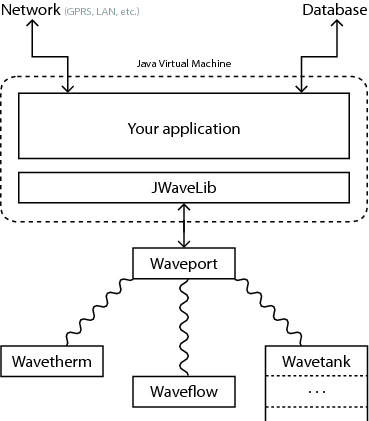
\includegraphics{schema.png}\hfill}

The following snippet shows how easy it can be

\begin{Verbatim}[commandchars=@\[\]]
import com.coronis.modules.platform.SerialWavePort;
import com.coronis.modules.WaveFlow;
import com.coronis.modules.WavePort;
import com.coronis.modules.WaveTherm;
// initialise Waveport
WavePort wpt = new SerialWavePort(“waveport1”, “/dev/ttyUSB0”);
// initialise a Wavetherm using no Wavetalk
JWaveLib WaveTherm wth1 = new WaveTherm(“031907301989”, wpt, null);
int temperature = wth1.getCurrentValue();
// initialise Waveflow using no Wavetalk
WaveFlow wfl1 = new WaveFlow(“021607314289”, wpt, null);
int index = wfl1.getCurrentValue();
DataSet dst = wfl1.getDailyData();
\end{Verbatim}


\chapter{Technical overview}
\label{technical_overview:technical-overview}\label{technical_overview::doc}
This chapter will give an overview of the JWaveLib architecture and implementation.


\section{History}
\label{technical_overview:history}
The JWaveLib has originally been developped to be integrated into embedded
Java hardware. The first running implentation was made for ACTL eWON's in 2007.
The application was designed to do some data acquisition at a given frequency.
Thus, the main development were focused on datalogging access. The library is
now opening to support all the types of communication a user can think about
using Coronis devices.

The JWaveLib is now running on different architectures from classic J2SE
environements to embedded platforms like the ACTL eWON or the Siemens TC65.


\section{Architectural details}
\label{technical_overview:architectural-details}
The JWaveLib hides all of the Wavenis protocol behind easy to use objects
(WavePort, WaveTherm, etc.). A rich set of exceptions are used through the
library allowing the user to catch and understand what the problem is.

Using the library is limited to declaring a WavePort instance, connecting them
to Modules (any Coronis module) and then using those modules. Depending on the
module type, a different set of methods are available.

If needed, existing module types can be extended to implement specific
functionalities.


\subsection{WavePort}
\label{technical_overview:waveport}
The \textbf{com.coronis.module.WavePort} class is the central point. It is in charge
of doing all the job of talking and listening to an RS-232 connected WavePort.
It offers the needed methods to do point-to-point or multiframe requests. Some
broadcasting queries have already been tested but not officialy implemented in
the library.

This class is abstract because dependant on the hardware.


\subsection{Module}
\label{technical_overview:module}
The \textbf{com.coronis.module.Module} class is the parent of all the Coronis modules
(WaveTalk or DataloggingModule). This class contains all the methods shared by
the different Coronis modules (get/set firmware, get type, get/set datetime,
etc.).

A Module has also references to a list of repeaters if any. This list of
repeaters will automatically be used to optimize the type of request between the
WavePort and the Module (PTP, Repeated or Multiframe).


\subsection{DataLoggingModule}
\label{technical_overview:dataloggingmodule}
The \textbf{com.coronis.module.DataLoggingModule} class allow management of modules that have datalogging tables (simple or extended).

The DataLoggingModule class is abstract as the methods reading the data from
the modules are module specific (e.g. WaveFlow stores the index information on
4 bytes while the WaveTherm Dallas stores information on 2 bytes). The specific
implementation are done inside the children classes :
\begin{itemize}
\item {} 
\textbf{com.coronis.module.WaveTherm},

\item {} 
\textbf{com.coronis.module.WaveFlow},

\item {} 
\textbf{com.coronis.module.WaveTank}

\item {} 
\textbf{com.coronis.module.WaveSense}

\end{itemize}

When retrieving data from the sensors, the methods returns
\textbf{com.dipole.libs.DataSet} objects that holds the retrieved information. a
DataSet is a list of \textbf{com.dipole.libs.Measure} objects and some metadata
about them (last call date, ...).

This class is the primary input point when the user would probably need to implement specific behaviour dependant on their need.


\section{Library packages}
\label{technical_overview:library-packages}
This section will describe each package of the library and will give a brief
overview of their content and use. For a more detailed information, please
refer to the javadoc.

The list of packages in the jwavelib.jar library :


\subsection{com.coronis}
\label{technical_overview:com-coronis}
General package holding classes shared all over the library


\subsection{com.coronis.exceptions}
\label{technical_overview:com-coronis-exceptions}
Exception package grouping a nice set of exception classes. The base class of all the exceptions is \textbf{CoronisException}.


\subsection{com.coronis.frames}
\label{technical_overview:com-coronis-frames}
Every incoming and outgoing Coronis frames are managed by this package. A factory frame builder (\textbf{CoronisFrameBuilder}) and a state machine frame reader (\textbf{CoronisFrameReader}) can read or produce any of the Coronis frames existing in this package.


\subsection{com.coronis.logging}
\label{technical_overview:com-coronis-logging}
The JWaveLib uses a logging module a la log4j but very light. Everything is based on the \textbf{SimpleLogger} interface. The \textbf{Logger} class uses only static methods and is used all over the library. By default, it uses a \textbf{StdLogger} that outputs all the logging to the standard output. Depending on the debugging configuration, the different levels of logging will print messages. The \textbf{frame()} method allows logging of Coronis frames.


\subsection{com.coronis.modules}
\label{technical_overview:com-coronis-modules}
The physical Coronis modules have a class counterpart. The base module is the \textbf{WavePort} and the connected module to the WavePort are all children of the \textbf{Module} class. The hierarch is the following :
\begin{itemize}
\item {} 
WavePort

\item {} 
Module

\end{itemize}
\begin{quote}
\begin{itemize}
\item {} 
WaveTalk

\item {} 
DataloggingModule

\end{itemize}
\begin{quote}
\begin{itemize}
\item {} 
WaveTherm

\end{itemize}
\begin{itemize}
\item {} 
WaveThermDallas

\item {} 
WaveThermPT100

\end{itemize}
\begin{itemize}
\item {} 
WaveFlow

\item {} 
WaveSense

\end{itemize}
\begin{itemize}
\item {} 
WaveSense4\_20

\item {} 
WaveSense5V

\item {} 
WaveTank

\end{itemize}
\end{quote}
\end{quote}


\subsubsection{com.coronis.modules.platform}
\label{technical_overview:com-coronis-modules-platform}

\subsubsection{com.coronis.modules.requests}
\label{technical_overview:com-coronis-modules-requests}

\subsection{com.dipole.libs}
\label{technical_overview:com-dipole-libs}

\section{Test packages}
\label{technical_overview:test-packages}

\subsection{com.coronis.test}
\label{technical_overview:com-coronis-test}

\section{Integrating JWaveLib}
\label{technical_overview:integrating-jwavelib}
From an integrator point of view, the JWaveLib provides easy extension points
by the use of abstract classes and the object orientation of the package :
\begin{itemize}
\item {} 
The hardware specific classes have all been made abstract to ensure each platform has its implentation of the classes.

\item {} 
When a user wants to implement specific methods, he can derive from existing classes to implement the new methods or overload existing ones

\end{itemize}


\chapter{Implementing the JWaveLib}
\label{implementation:implementing-the-jwavelib}\label{implementation::doc}
This chapter will list the implementation of the JWaveLib into different
architectures.


\section{Java 2 Standard Edition}
\label{implementation:java-2-standard-edition}
The JWaveLib is also supported by standard Java runtime environment. Using the
Java Communication API or the RXTX library, it can very easily be integrated in
any application to offer the full access to the Coronis modules.


\section{ACTL eWON implementation}
\label{implementation:actl-ewon-implementation}
This is the original development platform of the JWaveLib and as thus been
thorougly tested. This is the reference implementation of the JWaveLib.

The eWON SDK offered an easy interface to the JWaveLib. The development was mainly focused on interacting with the eWON (using the filesystem, GPRS, leds, etc.) as the JWaveLib integration was limited to implementing the WavePort abstract class for the eWON Java environment.

Further work is planned to allow more interactions with the eWON tags and other configuration.


\section{Siemens TC65 implementation}
\label{implementation:siemens-tc65-implementation}
The JWaveLib implementation into the TC65 has been tested in our lab but has
not been putted under production condition.


\chapter{Support}
\label{support:support}\label{support::doc}

\section{Bug reports}
\label{support:bug-reports}
For any bug reports, do ask a login to \href{mailto:support@dipole-consulting.com}{support@dipole-consulting.com} and report
the tickets onto the JWaveLib trac instance :
\begin{quote}

\href{http://svn.dipole-consulting.com/jwavelib/trac.cgi}{http://svn.dipole-consulting.com/jwavelib/trac.cgi}
\end{quote}

The trac is opened to all of your JWaveLib clients. If you require more
confidentiality, please report your bug by e-mail to
\href{mailto:support@dipole-consulting.com}{support@dipole-consulting.com}


\section{Technical assistance}
\label{support:technical-assistance}
For technical assistance, please contact the support by e-mail :
\href{mailto:support@dipole-consulting.com}{support@dipole-consulting.com}


\section{Frequently Asked Questions}
\label{support:frequently-asked-questions}
This section is a copy of the FAQ content you can find on the JWaveLib trac
instance.


\subsection{Supported features}
\label{support:supported-features}\begin{itemize}
\item {} 
What kind of Coronis modules have been fully tested using JWaveLib ?

\end{itemize}

The following list of modules have been thoroughly tested and are active on production sites :
\begin{enumerate}
\item {} 
WaveTherm Dallas - 1 sensor

\item {} 
WaveFlow - 1 counter

\item {} 
WaveTalk 25 mW and 500 mW

\item {} 
Serial WavePort 25/500 mW

\end{enumerate}
\begin{itemize}
\item {} 
What is the list of all the supported Coronis modules ?
\begin{enumerate}
\item {} 
WaveTherm Dallas - 1 sensor

\item {} 
WaveFlow - 1 counter

\item {} 
WaveTank

\item {} 
WaveTalk 25 mW and 500 mW

\item {} 
Serial WavePort 25/500 mW

\end{enumerate}

\item {} 
What if the modules I want to use is not already supported by the JWaveLib ?

\end{itemize}

Our politic is to support all the Coronis modules. Thus if you plan to use a module that is not actually supported by the JWaveLib, contact the support and we will give you an estimated time to get full support on this module. Lots of modules just require a very small development to work with the current JWaveLib.

For example : you need to use a WaveFlow? with two counters (A and B). Dipole Consulting will provide you a JWaveLib version supporting this type of module within one month.
\begin{itemize}
\item {} 
Does JWaveLib support automatic network configuration (SDP) ?

\end{itemize}

At the moment, JWaveLib does not support the SDP protocol. The feature is in the development process for milestone 2.0 if available in the Coronis modules. The SDP protocol is not already available into the Coronis modules.


\subsection{Configuration}
\label{support:configuration}

\subsection{Coronis products related questions}
\label{support:coronis-products-related-questions}\begin{itemize}
\item {} 
How can we know if the module supports extended datalogging ?

\end{itemize}

This is not possible using the Wavenis protocol. If the module has a strange behaviour when asking for the extended datalogging measures, it does probably not support extended datalogging. Only the Coronis technical support can confirm it. Send an e-mail with the module id to \href{mailto:technicalsupport@coronis.com}{technicalsupport@coronis.com} to check that.


\subsubsection{Waveport}
\label{support:waveport}

\subsubsection{Waveflow}
\label{support:waveflow}

\chapter{JWaveLib versions}
\label{version:jwavelib-versions}\label{version::doc}

\section{Version 1.0.2}
\label{version:version-1-0-2}\begin{itemize}
\item {} 
Released 11/21/2008

\item {} 
Important bugfix for extended datalogging parameters check

\item {} 
See changeset {[}15{]}

\end{itemize}


\section{Version 1.0.0}
\label{version:version-1-0-0}\begin{itemize}
\item {} 
Released 10/01/2008

\item {} 
First official release. Library used in production using eWon hardware on approximatively 30 sites.

\end{itemize}


\chapter{Contacts}
\label{contacts::doc}\label{contacts:contacts}
For any information, please contact :

\begin{DUlineblock}{0em}
\item[] \textbf{Dipole Consulting SPRL}
\item[] Rue d'Arnelle, 4
\item[] 1315 Incourt
\item[] Belgium
\item[] 
\item[] \href{mailto:info@dipole-consulting.com}{info@dipole-consulting.com}
\item[] +32 10 77 90 05
\item[] +32 475 665 668
\item[] 
\item[] \href{http://svn.dipole-consulting.com/jwavelib/trac.cgi}{http://svn.dipole-consulting.com/jwavelib/trac.cgi}
\item[] \href{http://www.dipole-consulting.com}{http://www.dipole-consulting.com}
\end{DUlineblock}



\renewcommand{\indexname}{Index}
\printindex
\end{document}
